\documentclass[..]{subfiles}


\begin{document}

\chapter{Protocol Properties}\label{chap:properties}

This chapters has two main sections. In the first section all necessary definitions and preliminary results are developed. In the second section the main properties of the Blockchain protocol described in Chapter \ref{chap:protocol} are defined, illustrated and proved. This chapter is mainly based on \cite{garay2015bitcoin}.


\section{Preliminaries}

In order to complete a PoW a party needs to find a value combination $H(\alpha, \rho, x)$ such that $H(\alpha, \rho, x) \le T$. A query in which such value is found will be called \textit{successful}.

\begin{definition}[Random Variables]
	\mbox{}\\
	\normalfont
	For every round $i \in \{1,\dots,\lambda\}$, query $j \in \{1,\dots,q\}$ and adversary $k \in \{1, \dots,t\}$ the following random variables are defined; If at round $i$ an honest party succeeds at solving POW, then $X_i = 1$, otherwise $X_i = 0$. If at round $i$ exclusively an honest party succeeds at solving POW, then $Y_i = 1$, otherwise $Y_i = 0$. If at round $i$, at query $j$ the adversary $k$ obtains a successful query, then $Z_{ijk} = 1$, otherwise $Z_{ijk} = 0$. Also $Z_i = \sum_{k=1}^{t}{\sum_{j=1}^{q}{Z_{ijk}}}$. Consequently, for a set of rounds $S$, $X(S) = \sum_{s \in S}{X_i}$, similarly for $Y(S)$ and $Z(S)$.
\end{definition}

A round such that $X_i = 1$ will be called a \textit{successful round}, a round such that $Y_i = 1$ will be called a \textit{uniquely successful round}. Now a set of events will be described. These events are extremely problematic since the possibility of their occurrence disrupts the plot of some proofs.

\begin{definition}[Disruptive Events]
	\mbox{}
	\normalfont

	\begin{itemize}
		\item An \textit{insertion} occurs when, given a chain which contains two consecutive blocks $B_1$ and $B_2$, a block $B_3$ is calculated such that $B_1, B_3, B_2$ constitute three consecutive blocks of a valid chain.
		\item A \textit{copy} occurs when the same block $B$ is present in two different positions.
		\item A \textit{prediction} occurs when a block extends one which was computed at a later round.
	\end{itemize}
\end{definition}

In our model(as long as the executions is polynomially bounded in $\kappa$) these events are extremely unlikely(their probability is exponentially small in $\kappa$). A typical execution is one in which these events do not occur and the sum of the random variables $X, Y, Z$ does not deviate too much from their expected value in any big enough subset of rounds.

\begin{definition}[Typical Execution]
	An execution is $(\epsilon, \lambda)$-typical, for $\epsilon \in (0,1)$ and $\lambda \in \N, \lambda \ge 2/f$, if, for any set $S$ of at least $\lambda$ consecutive rounds, the following hold:
	\begin{enumerate}[(a)]
		\item $(1 - \epsilon)\E[X(S)] < X(S) < (1 + \epsilon)\E(S)$.
		\item $(1 - \epsilon)\E[Y(S)] < Y(S)$.
		\item $Z(S) < \E[Z(S)] + \epsilon \E[X(S)]$.
		\item No disruptive events occurred.
	\end{enumerate}
\end{definition}

\begin{remark}
	The fact that a typical execution is only defined for $\lambda \ge 2/f$ may look arbitrary now but will be an important hypothesis in order to prove Lemma \ref{typical_condition}.
\end{remark}

\begin{theorem}
	An execution is typical with probability $1-e^{-\Omega(\epsilon ^2 \lambda f + \kappa - log(L))}$. Where $L$ is the total runtime of the system(the total number of rounds).
\end{theorem}

\begin{remark}
	\normalfont
	$\Omega$ notes a positive transformation and is used to stress the parameters of the probability of a typical execution and their relation while obscuring irrelevant constants. It is easy to see that $1-e^{-\Omega(\epsilon ^2 \lambda f + \kappa - log(L))}$ is negligible in $\kappa$ since functions $n \mapsto a^{-n}$  are negligible $\forall a \ge 2$.
\end{remark}


In order to bound the random variables expectancy a hypothesis on some parameters needs to be imposed. Let $f = \E[X_i]$, i.e, the possibility that at least one honest party solves POW at a given round.
\begin{definition}[Honest Majority Assumption]
	With respect to the number of adversaries $t$ out of the total number of parties $n$ the following inequality holds: $\frac{t}{n-t} \le (1-\delta)$, where $3f + 3\epsilon < \delta \le 1$.
\end{definition}
The first inequality encapsulates the fact at least half of the parties are honest. The second inequality will be essential in order to obtain an important bound. In essence it represents a trade-off between $f$ and $\epsilon$. $\epsilon$ can be seen as the \textit{quality of concentration of random values} in a run since it assures the number of successful and uniquely successful rounds is not far from their expected value and the number of adversary successful rounds is not much higher than its expected value. Particularly, it implies: $f,\epsilon < \frac{\delta}{3} \le \frac{1}{3}$ and $$(1+\epsilon)(1+f) < (1-\epsilon)(1-f)(1+\delta) < (1-\epsilon)(1-f)/(1-\delta)$$
For the first inequality $(1+\epsilon)(1+f) = 1+f+\epsilon+f\epsilon$ and $(1-\epsilon)(1-f)(1+\delta) = (1-\epsilon-f+f\epsilon)+((1-\epsilon)(1-f)\delta)$ hence, the inequality will hold if, and only if, $2\epsilon + 2f < (1-\epsilon)(1-f)\delta$. As $2\epsilon + 2f = 2(\epsilon + f) < \frac{2\delta}{3}$ if the following inequality is true so will be the last $\frac{2\delta}{3} < (1-\epsilon)(1-f)\delta \iff \frac{2}{3} < (1-\epsilon)(1-f) \iff 0 < (1-3(\epsilon-f) + 3f\epsilon)$ but $(1-3(\epsilon-f) + 3f\epsilon) > 1 - \delta + 3f\epsilon > 3f\epsilon > 0$.
For the second inequality $1+\delta<\frac{1}{1-\delta} \iff 1 - \delta^2 < 1$, which is true.

Now some bounds for the random variables expectations will be calculated and they will be used in order to calculate other bounds that are true in the context of a typical execution. $X_i \leadsto B(1,f)$ and $f=1 - (1-p)^{q(n-t)}$ where $p$ is the probability of a successful query. This is because there are $(n-t)$ honest parties, each of which has $q$ queries to the hash function every round, thus the probability of failing all of them is $(1-p)^{q(n-t)}$ and the probability of succeeding in one of them is the complementary event. On the other hand, $p=T/2^\kappa$ since out of all the possible outputs of the hash function only the smallest $T$ are valid. The following bounds on $\E[X_i]$ hold:
$$(1-f)pq(n-t) < f = \E[X_i] = 1 - (1-p)^{q(n-t)} < pq(n-t)$$
For the first inequality $e^rx \ge (1+x)^r$ for reals $x$ and $r \ge 0$ was used:
$$\frac{f}{1-f} = \frac{1 - (1-p)^{q(n-t)}}{(1-p)^{q(n-t)}} = (1-p)^{-q(n-t)} - 1 > e^{-q(n-t) - 1} - 1 \ge q(n-t) > pq(n-t)$$
For the second inequality Bernouilli's inequality was used $(1+x)^\alpha > 1 + \alpha x$ for reals $x > -1$ and $\alpha > 1$. Multiplying by $-1$ each member $-(1+x)^\alpha < -1 - \alpha x$:
$$1 - (1-p)^{q(n-t)} < 1-1-(-p)q(n-t) = pq(n-t)$$
The Bernouilli inequality was used with $x=-p$ and $\alpha = q(n-t)$.

The following bounds link $Y_i$ and $Z_i$ expectations to $f$. Related to $\E[Y_i]$:
$$\E[Y_i] \ge q(n-t)p(1-p)^{q(n-t)-1} > pq(n-t)[1 - pq(n-t)] > f(1-f) > \left(1-\frac{\delta}3\right)f$$
Since $Y_i$ is also a binomial distribution that models the probability that at a given round exactly one honest party solves POW its expectation will be at least the probability of all honest parties making all $q$ queries and failing all of them except one, hence the first inequality. For the second inequality, first a unity was added to the exponent, since $(1-p) < 1$ this makes for the strict inequality and second Bernouilli's inequality was used. For the third inequality:
\[ 
\left. \begin{array}{r} 
	\textrm{Function }x \mapsto x(1-x) \textrm{ is increasing in } (0,1/2)\\[1ex]
	f < pq(n-t) < f(1-f)^{-1} \underbrace{<}_\text{$f < \frac{\delta}{3}$} \frac{\delta}{3}(1-\frac{\delta}{3})^{-1} \underbrace{\le}_\text{$\delta \le 1$} \frac{1}{2}
\end{array} \right\} 
pq(n-t)[1 - pq(n-t)] > f(1-f)
\]
Finally, for the last inequality $1-f > 1-\delta$ was used. Note that the fact that $f < 1/3$ is actually essential since function $x \mapsto x(1-x)$ is not monotone(much less increasing) in any interval $(a, b)$ with $0 \le a \le 1/2 \le b$.

Lastly, since $Z_i$ models number of POW obtain by the adversary in a given round $Z_i \leadsto B(qt, p)$. Consequently, $\E[Z_i] = pqt$. Related to $\E[Z_i]$:
$$\E[Z_i] = pqt = pq(n-t) \frac{t}{n-t} <  \frac{f}{1-f} \cdot \frac{t}{n-t} < \left(1+\frac{\delta}{2}\right) \cdot f \cdot \frac{t}{n-t}$$
The first inequality is a consequence of the previous bounds and the second one is a consequence of: $\frac{1}{1-f} < \frac{1}{1-\frac{\delta}{3}} = 1 + \frac{\delta}{3-\delta}$ and $1 + \frac{\delta}{3-\delta} \le 1 + \frac{\delta}{2} \iff \frac{2}{3-\delta} \le 1 \iff \delta \le 1$.


Now the previous bounds will be used to achieve useful bounds based on the properties of a typical execution:
\begin{lemma}\label{typical_bounds}
	In a typical execution under the honest majority assumption, for any set S of at least $\lambda$ consecutive rounds it holds:
	\begin{enumerate}[(a)]
		\item $(1 - \epsilon)f|S| < X(S) < (1 + \epsilon)f|S|$.
		\item $(1 - \frac{\delta}{3})f|S| < (1 - \epsilon)f(1-f)|S| < Y(S)$.
		\item $Z(S) < \frac{t}{n-t} \cdot \frac{f}{1-f}|S| + \epsilon f|S| \le (1-\frac{2 \delta}{3})f|S| < (1-\frac{\delta}{2})X(S)$.
	\end{enumerate}
\end{lemma}
\mbox{}
\begin{proof}
	\mbox{}
	\begin{enumerate}[(a)]
		\item It is enough with $X(S) = \sum_{s \in S}{X_r} \Rightarrow X(S) \leadsto B(|S|,f)$, since $X_s \leadsto B(1,f), \forall s \in S$ and, therefore $\E[X(S)] = |S|f$.

		\item $\E[Y(S)] = \E[Y]|S|$ and $Y(S) > (1-\epsilon)\E[Y(S)] = (1-\epsilon)\E[Y]|S| > (1-\epsilon)f(1-f)|S| > (1-\epsilon)f(1-f)|S| = (1-\epsilon-f-f\epsilon)f|S| > (1-\frac{\delta}{3}+f\epsilon)f|S| > (1-\frac{\delta}{3})f|S|$. The rest follows from the bounds given at the beginning.

		\item As with the other random variables $\E[Z(S)] = \E[Z]|S|$. The first inequality is obtained substituting $\E[Z(S)]$ for its value and using one of the bounds for $\E[Z]$. The second inequality is obtained . The las inequality follows from the lower bound obtained in (a): $(1-\frac{2\delta}{3})f|S| < (1-\frac{2\delta}{3})\cdot \frac{1}{1-\epsilon} \cdot X(S) < (1-\frac{2\delta}{3})\cdot \frac{1}{1-\frac{\delta}{3}} \cdot X(S) = \left(\frac{3-2\delta}{3-\delta}\right) X(S) = \left(1 - \frac{\delta}{3-\delta}\right) X(S) < \left(1-\frac{\delta}{2}\right) X(S)$.
	\end{enumerate}
\end{proof}

\begin{remark}
	\normalfont
	From Lemma \ref{typical_bounds} it can be deducted that tuning $f$ value is a difficult task. $f = \E[X] = 1 - (1-p)^{q(n-t)}$, thus, it is a function of $q = T/2^\kappa$ which is a function of the security parameter $\kappa$ that can be changed during the course of the execution. The problem is, if $f$ is ``big'', then the concentration of random variable $X(S)$ will grow but $Y(S)$ will get hurt since $Y(S)$ depends on $1-f$ also the amount of adversary success $Z(S)$ will grow too. Since the adversary is supposed to have rushing capabilities this goes to his advantage and ends up causing him to make a bigger contribution on the chain damaging \textit{chain quality property} which will be soon defined. More in Remark \ref{rem:hurting_cq}. On the other hand, if $f$ is very ``small'', then the overall amount of successful queries will be small, including the adversary's. But this is also a problem, if successful queries are not frequent enough then the chain will not make progress and no new content is added to the chain which will get stuck hurting another property that will be soon defined known as \textit{chain growth property}. Thus, tuning $f$ is a compromise. In the Bitcoin network, such calibration takes places every 2016 blocks and attempts to keep $f$ in between $2-3\%$.
\end{remark}




\begin{corollary}\label{typical_race}
	In a typical execution under the honest majority assumption, for any set S of at least $\lambda$ consecutive rounds it holds:
	$Z(S) < Y(S)$.
\end{corollary}
\begin{proof}
	$Z(S) < (1-\frac{2\delta}{3})f|S| < (1-\frac{\delta}{3})f|S| < Y(S)$
\end{proof}

\begin{remark}
	\normalfont
	Corollary \ref{typical_race} is important because it states that there is no way for the adversary $\mathcal{A}$ to perpetrate a successful \textit{selfish mining} attack any a set of $S$ or more consecutive rounds of a typical execution under the honest majority assumption. A selfish mining attack is that in which a party attempts to withold one or more successfully calculated blocks from being broadcast to the rest of the parties. This is one of the most feared attacks in Blockchain literature and the only used in the naive analysis made by Nakamoto in his famous article \cite{nakamoto2008bitcoin}. Not only the adversary cannot win the race but it will clearly lose since only uniquely successful rounds are taken into consideration and successful rounds include uniquely successful rounds, thus, $Z(S) < Y(S) < X(S)$.
\end{remark}


\begin{lemma}\label{typical_condition}
	In a typical execution, any $k \ge 2 \lambda f$ consecutive blocks of a chain have been computed in more than $k/2f$ consecutive rounds.
\end{lemma}
\begin{proof}
	Assume there is a set of consecutive rounds $S'$ in which $K$ blocks were computed and assume $|S'|<\frac{k}{2f}$. Adding rounds to $S'$ makes it so the same amount of blocks or more are computed, as consequence let $S$ be a set of consecutive rounds with $|S| = \lceil\frac{k}{2f}\rceil + 1$ hence $X(S) + Z(S) \ge k$. But this is a contradiction since
	$$X(S) + Z(S) < (2 + \epsilon - \frac{2\delta}{3}) f|S| \le (2 - 2f)f|S| \le (1-f)(k+4f) < k$$
	For the first inequality the bounds from Lemma \ref{typical_bounds} (a) and (b) were used\footnote{Lemma \ref{typical_bounds} can be used since $\lceil\frac{k}{2f}\rceil \ge \lambda$}. For the second inequality the honest majority assumption was used $3f + 3\epsilon < \delta \Leftrightarrow 3\epsilon -\ \delta < -3f \Longrightarrow 2 + \epsilon - \frac{2\delta}{3} = 2 + \frac{3\epsilon -2\delta}{3} < 2-\frac{3f + \delta}{3} < 2 - \frac{3f + 3f}{3} = 2 - 2f$. For the third inequality $|S| = \lceil\frac{k}{2f}\rceil + 1 \le \frac{k}{2f} + 2$. Finally the last inequality can be checked directly $(1-f)(k+4f) < k \Leftrightarrow K+4f-fk-4f^2 < k \Leftrightarrow 4f < fk + 4f^2 \Leftrightarrow 4 < k + f^2$ and the last inequality is true since $\frac{k}{2f} \ge \lambda \ge 2/f \Rightarrow k \ge 4$.
\end{proof}

\begin{remark}
	\normalfont
	Lemma \ref{typical_condition} basically states that in a typical execution apply for every set of $3\lambda f$ or more consecutive blocks. Given a chain $C$, at first glance, no one can tell how many rounds were needed for a subset of blocks to be calculated this is a problem since it will be necessary to apply Lemma \ref{typical_bounds} in order some relevant properties. Lemma \ref{typical_condition} is very important because it offers a one way relation between round number and consecutive block number making it feasible to use properties of a typical execution in a big enough subset of consecutive blocks which, contrary to rounds, can be counted just by looking at the chain. 
\end{remark}




\section{Chain Growth Property}

The first property to be defined is the \textit{common prefix property} parameterized by $s \in \N$ and $\tau \in (0, 1)$. This property states that in a fixed amount of rounds all honest parties chains will grow proportionally to the number of rounds considered, no matter what the adversary does. This is very important in order to assure chains make progress and, thus, new content keeps being added to the chain.

\begin{definition}[Chain Growth Property]
	\normalfont
	The \textit{chain growth} property with parameters $\tau \in (0, 1)$ and $s \in \N$ states that for any honest party $P$ that has a chain $\C$ in $\texttt{VIEW}_{\Pi, \mathcal{A}, \mathcal{Z}}^{t, n}$, it holds that after any s consecutive rounds it adopts a chain that is at least $\tau \cdot s$ blocks longer than $\C$.
\end{definition}

\begin{figure}[h]
	\begin{center}
		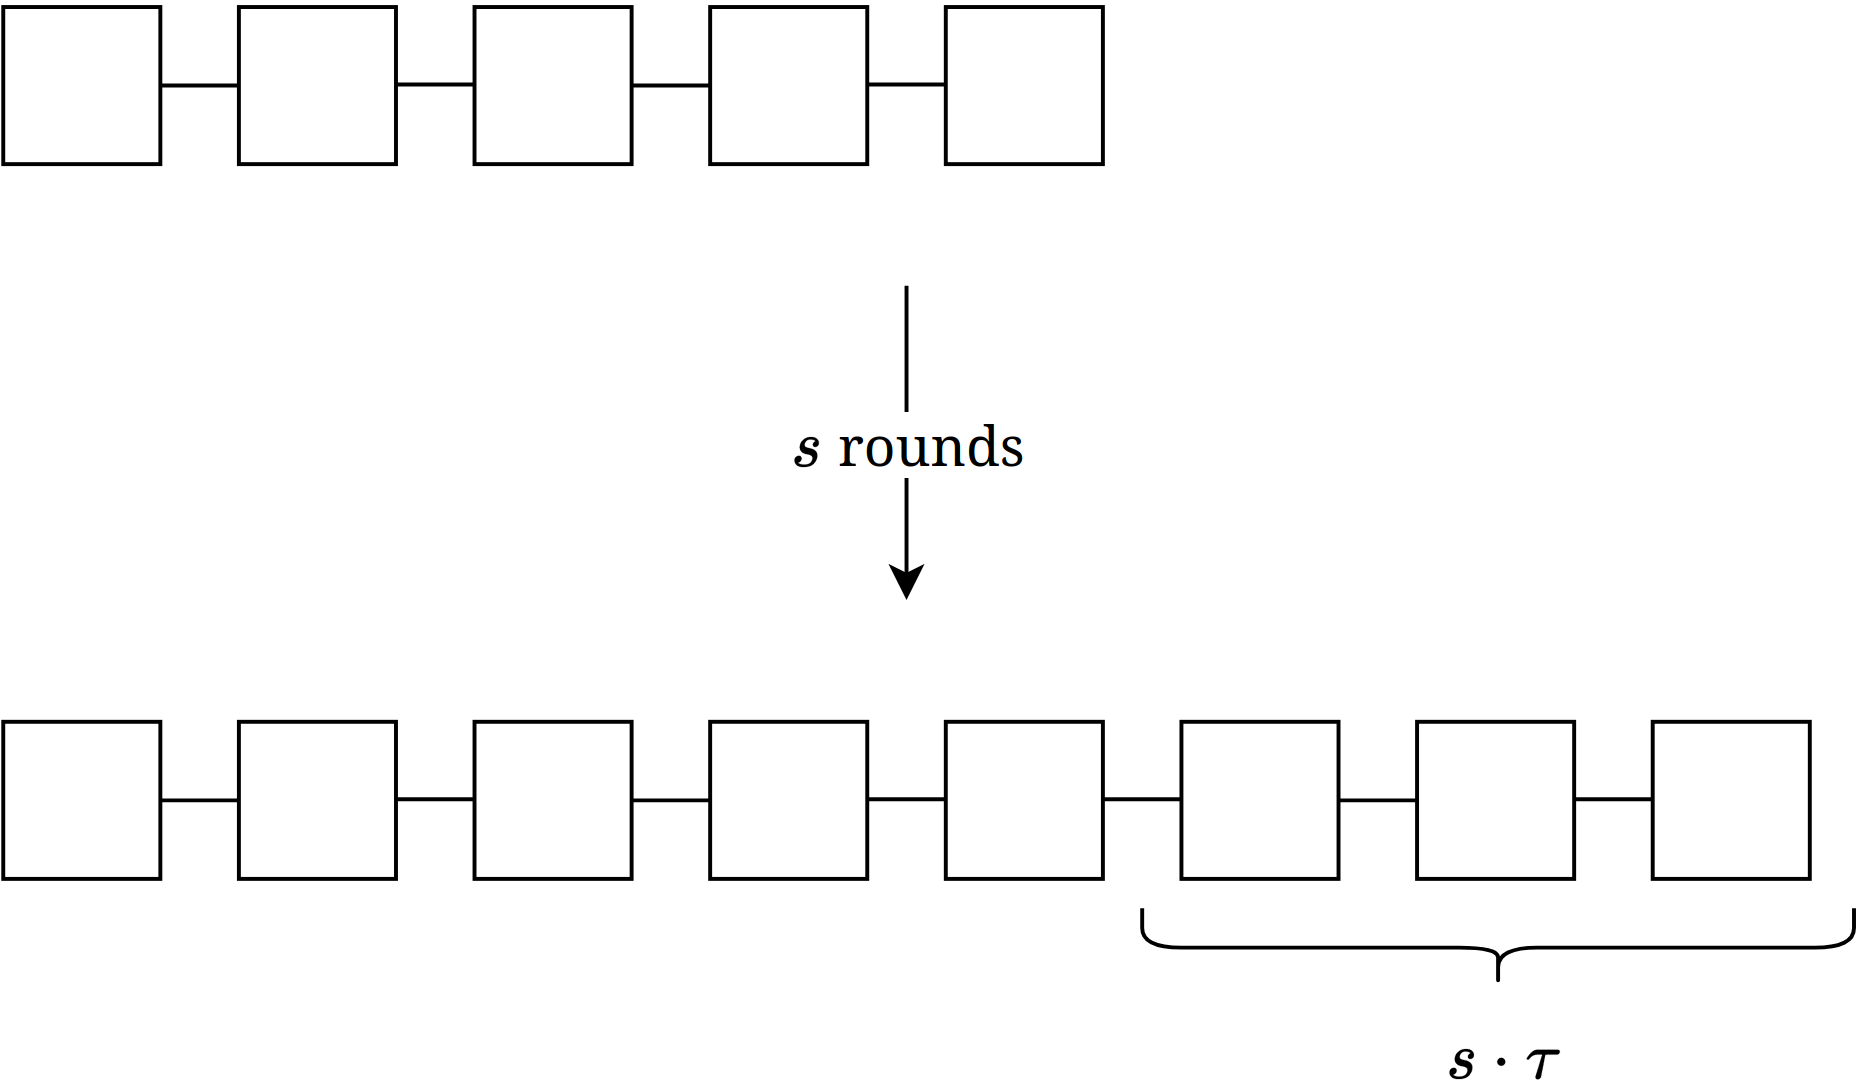
\includegraphics[width=0.85\textwidth]{figures/chain_growth.png}
	\end{center}
	\caption{Chain growth property sketch}
	\label{fig:cg}
\end{figure}


The following lemma states that, at any given round, the chain length of any honest party will be at least the sum of the number of successful rounds. This implies that the growth of the honest parties' chains will be at least the rate of the successful rounds independently of what the opponent does.
\begin{lemma}[Chain Growth Lemma]\label{cg_lemma}
	Suppose that at round $r$ an honest party has a chain of length $l$. Then, by round $s \ge r$, every honest party has adopted a chain of length at least $l + \sum_{i=r}^{s-1}{X_i}$.
\end{lemma}
\begin{proof}
	By induction on $s-r \ge 0$. For the base case $s=r$, if an honest party has a chain $C$ of length $l$, then that chain $C$ must have been broadcast at a round earlier that $r$, thus, all honest parties must have received $C$.
	For the inductive step, by the inductive hypothesis by round $s-1$ every honest party has received a chain $C$ of length $l + \sum_{i=r}^{s-2}{X_i}$. At round $s$, if $X_{s-1}(S) = 0$ there is nothing to do. If $X(S)_{s-1} = 1$, then some honest party achieved PoW and hence, broadcast a chain of length $l' + 1$, but since $l' = l + \sum_{i=r}^{s-2}{X_i} \Rightarrow l' + 1 = l + \sum_{i=r}^{s-1}{X_i}$.
\end{proof}

\begin{theorem}[Chain Growth]
	In a typical execution the chain growth property holds with parameters $\tau = (1 - \epsilon)f$ and $s \ge \lambda$.
\end{theorem}
\begin{proof}
	Suppose that at round $r$ an honest party has a chain $C$ of length $l$. Then, by round, $s$ it will have a chain of length, at least, $l + X(S)$ where $S$ represents the $s$ rounds following $r$, i.e, $S = \{i: r \le i < r+s\}$. Now, $|S| \ge \lambda$ by hypothesis and Lemma \ref{typical_bounds}(a) applies $X(S) > \underbrace{(1-\epsilon)f}_\text{$\tau$} \cdot \underbrace{|S|}_\text{s}$.
\end{proof}




\section{Common Prefix Property}

The second property considered is the \textit{common prefix property} parameterized by $k \in \N$. This property states that given an honest node chain any honest node's chain in a later round will share at least the first $k$ blocks with it. This property is very important because it assures that the parties are working on a common substratum that will never be altered, thus, their work is not in vain. 

\begin{definition}[Common Prefix Property]
	\normalfont
	The \textit{common prefix} property with parameter $k \in \N$ states that for any pair of honest players $P_1,P_2$ adopting the chains $\C_1,\C_2$ at rounds $r_1 \le r_2$ in $\texttt{VIEW}_{\Pi, \mathcal{A}, \mathcal{Z}}^{t, n}$ respectively, it holds that $\C_1^{\lceil k} \preceq \C_2$
\end{definition}

\begin{figure}[H]
	\begin{center}
		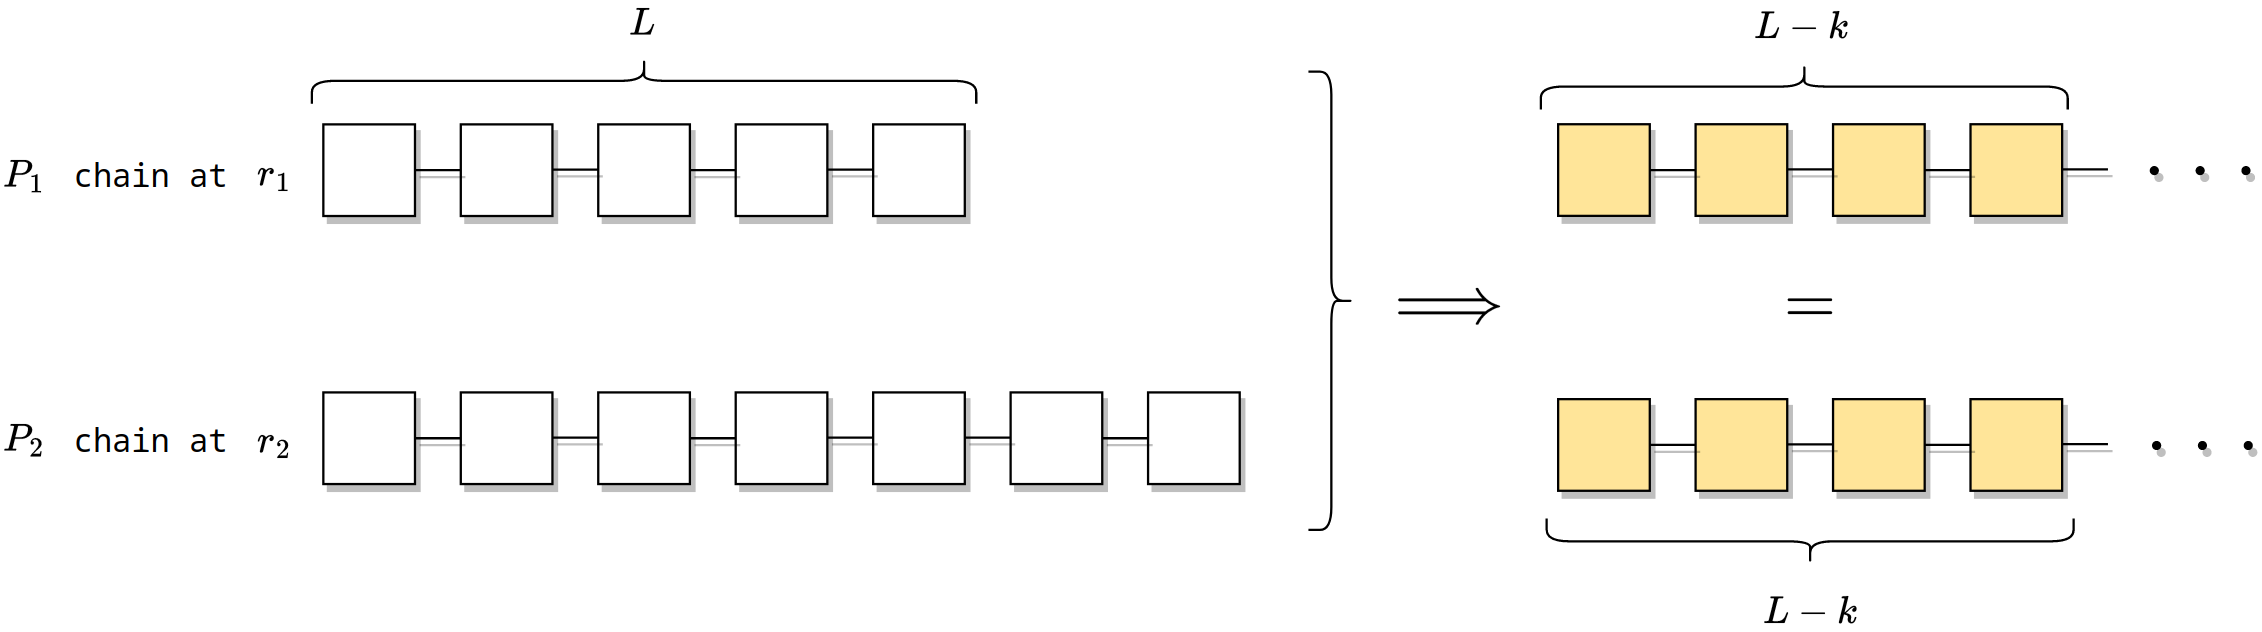
\includegraphics[width=0.98\textwidth]{figures/common_prefix.png}
	\end{center}
	\caption{Chain common prefix sketch}
	\label{fig:cp}
\end{figure}

\begin{definition}[Block types]
	\normalfont
	A block is said to be \textit{honest} if it was \textbf{computed and diffused} by an honest party and is said to be \textit{adversary} if it was \textbf{diffused} by the adversary.\footnote{This definition avoids controversy in demonstration of Lemma \ref{cp_lemma}}
\end{definition}

\begin{lemma}\label{us_property}
	Suppose the k-th block B of a chain $\C$ was computed by an honest party in a uniquely successful round. Then the k-th block a chain $\C'$ either is B or has been computed by the adversary.
\end{lemma}
\begin{proof}
	Suppose an honest block $B'$ is the k-th block in an honest party's chain $C'$. Also, suppose $B'$ is different from $B$. Let $r$ be the round when $B$ was calculated. Since $r$ is a uniquely successful round $B'$ had to be computed at a different round. But it cannot be computed at a later round: By Lemma \ref{cg_lemma}, at the beginning of $r$, every honest party's chain's length was the same $k-1$. Since $r$ is a uniquely successful round, during $r$ only one honest party calculated a new block and then broadcast its extended chain of length $k$. Every honest block calculated at a later round will be extending a chain of length more than $k$. It also couldn't be computed before: since a block is calculated upon a previous one if an honest party calculated a block in extending the $k-1$-th block of its chain it would broadcast it at the end of the round and all blocks calculated at a later round would be extending a chain of length $k$, particularly at round $r$. This contradicts the hypothesis "$B$ is the $k$-th block of a chain at round $r$".
\end{proof}

\begin{lemma}[Common Prefix Lemma]\label{cp_lemma}
	Suppose that at round $r$ of a typical execution an honest party has a chain $C_1$ and an honest party adopts a chain $C_2$ of length at least $len(C_1)$, then $C_1^{\lceil k} \preceq C_2$ and $C_2^{\lceil k} \preceq C_1$ for every $k \ge 2\lambda f$. 
\end{lemma}
\begin{proof}
	The proof is by contradiction. Assume that, in a typical execution, for some $k \ge 2\lambda f$, either $C_1 \npreceq C_2$ or $C_2 \npreceq C_1$. Let $r*$ be the round at which the last honest block of $C_1$s and $C_2$s common prefix was computed. If no such block exists let $r*=0$. Let $S = \{i : r* < i < r\}$, i.e, the set of rounds between $r* $ and $r$. It will be proved that
	$$Z(S) \ge Y(S)$$
	In order to prove it each block calculated in a uniquely successful round will be paired with an adversary block.
	
	First note that if the block mined at $r*$ occupies position $l$ then every block calculated in $S$ must extend a chain of length at least $l$. Now, for each uniquely successful round $u \in S$ let $j_u$ be the chains position of the block calculated at round $u$. Consider $P = \{p_u : u \textrm{ is uniquely succesful in } S\}$. Note that at round $r$ both chains have length at least $max(P)$. Therefore, for each $j \in J$ there is a block in position $p$ of both chains. Note that $P \neq \emptyset$ since trivially $Z(S)\ge0$. Now it will be proved that for each $p \in P$ at least one of the blocks in position $p$ is an adversary block.
	\begin{itemize}
		\item $p$ is on the common prefix: for being in the common prefix both block are equal, if the block was honest it would contradict $r*$ definition since every block calculated in $S$ is calculated after $r*$ but then, as noted before, there would exist a common honest block in position $j>l$, hence the block calculated in $r*$ would not be the last common honest block.
		\item $p$ is not on the common prefix: if there are two honest blocks in position $p$ then, by Lemma \ref{us_property} they must be equal, furthermore, there would be a common prefix of length $p$ since when the block is broadcast the complete chain is broadcast with it. This a contradiction with $p$ not being in the common prefix.
	\end{itemize}
	Last, by $C_1 \npreceq C_2$ or $C_2 \npreceq C_1$ for some $k \ge 2\lambda f$, $len(C_1) - l > k$ or $len(C_2) - l > k$, in any case, $l > 2\lambda f$ and, by Lemma \ref{typical_condition}, the properties of a typical execution apply. Particularly, by Corollary \ref{typical_race}, $Z(S) < Y(S)$.
\end{proof}


\begin{theorem}[Common Prefix]
	In a typical execution the common prefix property holds with parameter $k \ge 2 \lambda f$.
\end{theorem}
\begin{proof}
	Asume, towards a contradiction, chains $C_1$ and $C_2$ are adopted by parties $P_1$ and $P_2$ in rounds $r_1$ and $r_2$ such that $\C_1^{\lceil k} \npreceq \C_2$. By Lemma \ref{cp_lemma} in $r_1$ every honest parties chain contains $\C_1^{\lceil k}$, thus, there must be a round $r_1 \le r \le r_2$ in which an honest party $P$ has a chain $C$ containing $\C_1^{\lceil k}$ and adopts a another chain $C'$ such that $\C_1^{\lceil k} \npreceq C'$. Now, $C^{\lceil k} \npreceq C'$ and $len(C') \ge len(C)$, contradicting Lemma \ref{cp_lemma}.
\end{proof}
Note that, in the proof, $P$ doesn't have to be $P_2$ since the $C_2$ may have been built by a variety of different parties.



\section{Chain Quality Property}

The last property considered is the \textit{chain quality} parameterized by $\mu \in (0, 1)$ and $l \in \N$. This property states that at least a portion $\mu$ in any subset of length $l$ of consecutive blocks of any honest party's chain is made up of honest blocks. This property is important since it assures the contribution of the honest parties to the chain is high which in turn means that the impact of the adversary is limited.

\begin{definition}[Chain Quality Property]
	\normalfont
	The \textit{chain quality} property with parameters $\mu \in (0,1)$ and $l \in \N$ states that for any honest party P with chain $\C$ in $\texttt{VIEW}_{\Pi, \mathcal{A}, \mathcal{Z}}^{t, n}$, it holds that for any $l$ consecutive blocks of $\C$ the ratio of honest blocks is at least $\mu$.
\end{definition}

\begin{figure}[h]
	\begin{center}
		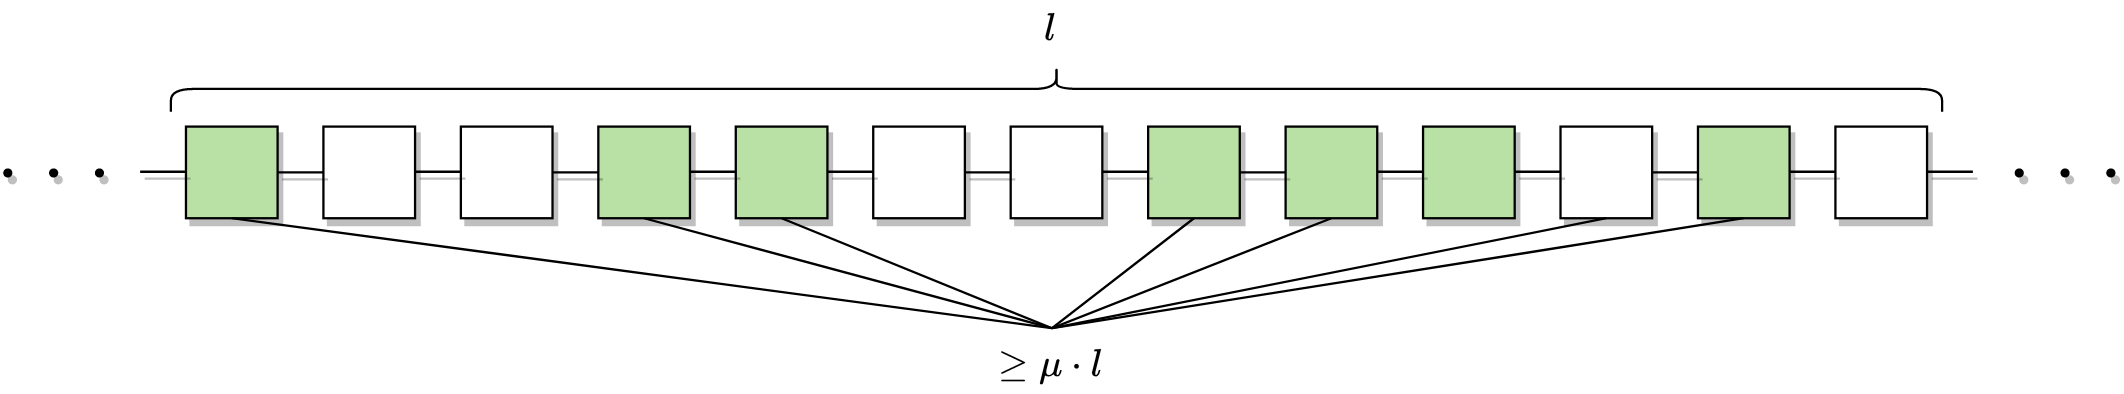
\includegraphics[width=0.98\textwidth]{figures/chain_quality.png}
	\end{center}
	\caption{Chain quality property sketch}
	\label{fig:cq}
\end{figure}

\begin{theorem}[Chain Quality]\label{theorem:cq}
	In a typical execution the chain quality property holds with parameters $l \ge 2 \lambda f$ and $\mu = 1 - (1+\frac{\delta}{2}) \cdot \frac{t}{n-t} - \frac{\epsilon}{1-\epsilon} > 1 - (1+\frac{\delta}{2}) \cdot \frac{t}{n-t} - \frac{\delta}{2}$.
\end{theorem}
\begin{proof}
	Let $B_k$ be the $k$-th block of a chain $C$ of an honest party $P$ at some round $r$ so that $C = B_1 \dots B_len(C)$ and consider $l$ consecutive blocks $B_i,\dots,B_j$. Let $L$ be the smallest set of consecutive rounds that include the $l$ given blocks (i.e $i' \le i$ and $j \le j'$) such that:
	\begin{enumerate}
		\item $B_i$ was computed by an honest party. If no such block exist the genesis block $B_1$ is taken.
		\item There exists a round at which an honest party was trying to extend the chain ending at block $B_j$. This is well defined since $B_{len(C)}$ is always at the head of a chain an honest party is trying to extend.
	\end{enumerate}
	Let $r_1$ be the round at which $B_{i'}$ was created ($r=0$ for $(B_1)$), let $r_2$ be the first round an honest party tried to extend $B_{j'}$ and let $S = \{r: r_1 \le r \le r_2\}$.

	Take $\mu$ as in the statement and let $x$ be the number of honest blocks in the $l$ selected blocks. Towards a contradiction assume that $$\mu L \ge \mu l > x$$
	Suppose that the $L$ blocks were computed during the rounds in $S$. Then
	$$Z(S) = L - x > (1-\mu)L \ge (1-\mu)X(S) =  \left(\left(1+\frac{\delta}{2}\right) \cdot \frac{t}{n-t} + \frac{\epsilon}{1-\epsilon}\right)X(S)$$
	The first inequality comes from $-x > -\mu L$. For the second inequality, suppose $X(S) > L$. At round $r_1$ an honest party produced $B_i'$ and therefore has a chain of length $i'$. By Lemma \ref{cg_lemma}, at round $r_2$ every honest party will have a chain of length $i' + X(S) > i' + L = j' + 1 > j'$ which is a contradiction.
	Finally, by Lemma \ref{typical_condition} $|S| \ge \lambda$ and the bounds of a typical execution apply, hence
	$$Z(S) \ge \left(\left(1+\frac{\delta}{2}\right) \cdot \frac{t}{n-t} + \frac{\epsilon}{1-\epsilon}\right)X(S) \ge \left(1 + \frac{\delta}{2}\right) \cdot \frac{t}{n-t} \cdot X(S) + \epsilon f |S| > Z(S)$$
	The second inequality uses Lemma \ref{typical_bounds} (a) and the third inequality uses Lemma \ref{typical_bounds} (c). The contradiction comes from supposing all blocks in $L$ have been computed during the rounds in $S$ and the relation between $x$ and $L$.

	If $L$ contains blocks calculated in rounds not in $S$. By the way $L$ is defined these blocks must have been computed by the adversary. If a block was calculated before $S$ then in order to belong to $L$ there would need to be a copy or a prediction since, the alternative would be the adversary building a chain of length bigger than $i'$ before the round $B_{i'}$ was calculated, but this would contradict $B_{i'}$ definition since when the adversary released its chain the block at position $i$ would be necessarily adversary. If a block was calculated after $S$ but still belongs to $L$ then there would need to be an insertion since otherwise the adversary would have to attempt to substitute one of the blocks in $L$ by outgrowing the honest chain beginning at any position in $L$, but this is a contradiction with the definition of $B_{j'}$ since when such chain was broadcast the last block in $L$ would not comply with its requirement of being worked on an extension by an honest node. As seen any of the possibilities requires a disruptive event that do not occur in a typical execution. The contradiction comes from assuming a block in $L$ has been computed in a round not in $S$ and the relation between $x$ and $L$.

	Adding both facts there is a contradiction with the relation between $x$ and $L$ which proves the theorem.
\end{proof}


\begin{corollary}
	Any $\lceil 2 \lambda f \rceil$ consecutive blocks in the chain of an honest party during a typical execution contain at least one honest block.
\end{corollary}
\begin{proof}
	$\mu = 1 - (1 + \frac{\delta}{2} \cdot \frac{t}{n-t} - \frac{\epsilon}{1-\epsilon}) \underbrace{>}_\text{$\epsilon < \frac{\delta}{3}$} 1 - (1 + \frac{\delta}{2}) \cdot \frac{t}{n-t} - \frac{\delta}{2} \underbrace{\ge}_\text{$\frac{t}{n-t} \le (1-\delta)$} 1 - (1 + \frac{\delta}{2}) \cdot (1-\delta) - \frac{\delta}{2} = 1 - [1 + \frac{\delta}{2} - \delta - \frac{\delta^2}{2}] - \frac{\delta}{2} = \frac{\delta^2}{2} > 0$
\end{proof}

\begin{remark}\label{rem:hurting_cq}
	\normalfont
	It can argued(informally) that Theorem \ref{theorem:cq} is tight under the hypothesis that chain ties always favor the adversary. This lies in the description of function \texttt{maxValid} and the fact that, in the considered model, the adversary has rushing capabilities, thus, they can get to write their chain in the input tape of every party before any honest party gets to diffuse its message. When the number of parties is large, in a round where an honest party finds a solution and the Adversary too(or had already found one) all other honest parties will prefer the adversary's chain and the effect of a single honest party opting for its own block is negligible.

	The attack that is going to be described a type of selfish mining attack that reaches the stated bound. Initially, the adversary works on the same chain as every honest party. However, when it finds a solution it keeps it to itself and continuous to extend its private chain. When an honest party finds a solution the adversary makes use of their rushing capabilities in order to release the first private block from their chain causing al honest parties to adopt it. This strategy maximizes the adversarial blocks in the Blockchain up to the upper bound of Theorem \ref{theorem:cq}.
	 
	Consider a set $S$ of consecutive rounds. With constant probability, in this set of rounds, the adversary will obtain, at least $z \ge pqt|S|$ solutions, while the honest parties will obtain at least $pq(n-t)|S| > x$ solutions. By following the detailed strategy the adversary can manage to counter(with overwhelming in $n$) $z$ out of $x$ honest blocks. Now, for the smallest sequence of blocks that contains the $z$ adversary blocks: $\mu \ge \frac{(x-z)}{x} = \frac{(n-2t)}{(n-t)} \ge 1 - (1+\frac{\delta}{2}) \cdot \frac{t}{n-t} - \frac{\epsilon}{1-\epsilon}$ for any $\delta, \epsilon \in (0, \frac{1}{3})$.

	From the above, in order to improve on chain quality a more favorable(for honest parties) tie breaking criteria needs to be considered. This translates in a need for a better connected network in which the adversary doesn't have such an strong capability as rushing or it is diminished in one way or another.
\end{remark}


\end{document}

